\documentclass[11pt]{article}
\usepackage[letterpaper, margin=1in]{geometry}
% \documentclass[useAMS,usenatbib,referee]{biomweb}
\usepackage{amssymb, amsthm, amsmath}
\usepackage{bm}
\usepackage{graphicx}
\usepackage[authoryear]{natbib}
\usepackage{bm}
\usepackage{verbatim}
\usepackage{lineno}
\usepackage{soul}
\usepackage[usenames, dvipsnames]{color}
% \usepackage{enumitem}
\usepackage{enumerate}
\usepackage{setspace}
\usepackage{appendix}
% \usepackage{caption}
% \captionsetup[table]{name=Web Table}

% cross-referencing appendices
\definecolor{wp-red}{RGB}{204,0,0}
\definecolor{wp-gray}{RGB}{51,51,51}
\definecolor{reynolds-red}{RGB}{153,0,0}
\definecolor{pyroman-flame}{RGB}{209,81,34}
\definecolor{hunt-yellow}{RGB}{253,215,38}
\definecolor{genomic-green}{RGB}{125,140,31}
\definecolor{innovation-blue}{RGB}{66,126,147}
\definecolor{bio-indigo}{RGB}{65,86,161}

\graphicspath{{../Chapter-2/plots/}{../Chapter-3/plots/}{../Chapter-4/plots/}{./plots/}}

% \usepackage[left=1in,top=1in,right=1in]{geometry}
% \pdfpageheight 11in
% \pdfpagewidth 8.5in
% \linespread{2.0}
\newcommand{\btheta}{ \mbox{\boldmath $\theta$}}
\newcommand{\bmu}{ \mbox{\boldmath $\mu$}}
\newcommand{\balpha}{ \mbox{\boldmath $\alpha$}}
\newcommand{\bbeta}{ \mbox{\boldmath $\beta$}}
\newcommand{\bdelta}{ \mbox{\boldmath $\delta$}}
\newcommand{\blambda}{ \mbox{\boldmath $\lambda$}}
\newcommand{\bgamma}{ \mbox{\boldmath $\gamma$}}
\newcommand{\brho}{ \mbox{\boldmath $\rho$}}
\newcommand{\bpsi}{ \mbox{\boldmath $\psi$}}
\newcommand{\bepsilon}{ \mbox{\boldmath $\epsilon$}}
\newcommand{\bomega}{ \mbox{\boldmath $\omega$}}
\newcommand{\bOmega}{ \mbox{\boldmath $\Omega$}}
\newcommand{\bDelta}{ \mbox{\boldmath $\Delta$}}
\newcommand{\bSigma}{ \mbox{\boldmath $\Sigma$}}
\newcommand{\bPsi}{ \mbox{\boldmath $\Psi$}}
\newcommand{\bLambda}{ \mbox{\boldmath $\Lambda$}}

% \newcommand{\btheta}{\ensuremath{\mathbf{\theta}}}
% \newcommand{\bmu}{\ensuremath{\mathbf{\mu}}}
% \newcommand{\balpha}{\ensuremath{\mathbf{\alpha}}}
% \newcommand{\bbeta}{\ensuremath{\mathbf{\beta}}}
% \newcommand{\bdelta}{\ensuremath{\mathbf{\delta}}}
% \newcommand{\blambda}{\ensuremath{\mathbf{\lambda}}}
% \newcommand{\bgamma}{\ensuremath{\mathbf{\gamma}}}
% \newcommand{\brho}{\ensuremath{\mathbf{\rho}}}
% \newcommand{\bpsi}{\ensuremath{\mathbf{\psi}}}
% \newcommand{\bepsilon}{\ensuremath{\mathbf{\epsilon}}}
% \newcommand{\bomega}{\ensuremath{\mathbf{\omega}}}
% \newcommand{\bOmega}{\ensuremath{\mathbf{\Omega}}}
% \newcommand{\bDelta}{\ensuremath{\mathbf{\Delta}}}
% \newcommand{\bSigma}{\mbox{\boldmath $\Sigma$}}
% \newcommand{\bPsi}{\ensuremath{\mathbf{\Psi}}}
\newcommand{\bOne}{\ensuremath{\mathbf{1}}}
\newcommand{\bZero}{\ensuremath{\mathbf{0}}}

\newcommand{\omu}{\overline{\mu}}
\newcommand{\oSigma}{\overline{\Sigma}}
\newcommand{\Yt}{{\tilde Y}}
\newcommand{\alphahat}{\hat{\alpha}}

\newcommand{\bA}{\ensuremath{\mathbf{A}}}
\newcommand{\bB}{\ensuremath{\mathbf{B}}}
\newcommand{\bb}{\ensuremath{\mathbf{b}}}
\newcommand{\bfe}{\ensuremath{\mathbf{e}}}
\newcommand{\bG}{\ensuremath{\mathbf{G}}}
\newcommand{\bH}{\ensuremath{\mathbf{H}}}
\newcommand{\bh}{\ensuremath{\mathbf{h}}}
\newcommand{\bI}{\ensuremath{\mathbf{I}}}
\newcommand{\bL}{\ensuremath{\mathbf{L}}}
\newcommand{\bk}{\ensuremath{\mathbf{k}}}
\renewcommand{\bm}{\ensuremath{\mathbf{m}}}
\newcommand{\bo}{\ensuremath{\mathbf{o}}}
\newcommand{\bP}{\ensuremath{\mathbf{P}}}
\newcommand{\bR}{\ensuremath{\mathbf{R}}}
\newcommand{\br}{\ensuremath{\mathbf{r}}}
\newcommand{\bs}{\ensuremath{\mathbf{s}}}
\newcommand{\bt}{\ensuremath{\mathbf{t}}}
\newcommand{\bu}{\ensuremath{\mathbf{u}}}
\newcommand{\bV}{\ensuremath{\mathbf{V}}}
\newcommand{\bv}{\ensuremath{\mathbf{v}}}
\newcommand{\bW}{\ensuremath{\mathbf{W}}}
\newcommand{\bw}{\ensuremath{\mathbf{w}}}
\newcommand{\bX}{\ensuremath{\mathbf{X}}}
\newcommand{\bx}{\ensuremath{\mathbf{x}}}
\newcommand{\bY}{\ensuremath{\mathbf{Y}}}
\newcommand{\by}{\ensuremath{\mathbf{y}}}
\newcommand{\bZ}{\ensuremath{\mathbf{Z}}}
\newcommand{\bz}{\ensuremath{\mathbf{z}}}

\newcommand{\iid}{\stackrel{\mathrm{iid}}{\sim}}
\newcommand{\ind}{\stackrel{\mathrm{ind}}{\sim}}
\newcommand{\dd}{\; \text{d} }
\newcommand{\ddd}{\text{d} }
\newcommand{\indep}{\stackrel{\text{indep}}{\sim}}
\newcommand{\converged}{\stackrel{\mathrm{d}}{\rightarrow}}
\newcommand{\calR}{{\cal R}}
\newcommand{\calG}{{\cal G}}
\newcommand{\calD}{{\cal D}}
\newcommand{\calS}{{\cal S}}
\newcommand{\calB}{{\cal B}}
\newcommand{\calA}{{\cal A}}
\newcommand{\calT}{{\cal T}}
\newcommand{\calO}{{\cal O}}
\newcommand{\argmax}{{\mathop{\rm arg\, max}}}
\newcommand{\argmin}{{\mathop{\rm arg\, min}}}
\newcommand{\Frechet}{\mbox{Fr$\acute{\mbox{e}}$chet }}
\newcommand{\Matern}{\mbox{Mat$\acute{\mbox{e}}$rn }}
\newcommand{\ballunion}{B_a(\bs_1) \cup B_b(\bs_2) }
\newcommand{\skewt}{\mbox{skew-\emph{t}}}
\newcommand{\Skewt}{\mbox{Skew-\emph{t}}}
\newcommand{\tamarix}{\emph{Tamarix ramosissima}}
\newcommand{\hedysarum}{\emph{Hedysarum scoparium}}


\newcommand{\beq}{ \begin{equation}}
\newcommand{\eeq}{ \end{equation}}
\newcommand{\beqn}{ \begin{eqnarray}}
\newcommand{\eeqn}{ \end{eqnarray}}

\newcommand{\eref}[1]{(\ref{#1})}
\newcommand{\fref}[1]{Figure~\ref{#1}}
\newcommand{\tref}[1]{Table~\ref{#1}}
\newcommand{\sref}[1]{Section~\ref{#1}}
\newcommand{\aref}[1]{Appendix~\ref{#1}}
\newcommand{\cref}[1]{Chapter~\ref{#1}}

\newcommand*\patchAmsMathEnvironmentForLineno[1]{%
  \expandafter\let\csname old#1\expandafter\endcsname\csname #1\endcsname
  \expandafter\let\csname oldend#1\expandafter\endcsname\csname end#1\endcsname
  \renewenvironment{#1}%
     {\linenomath\csname old#1\endcsname}%
     {\csname oldend#1\endcsname\endlinenomath}}%
\newcommand*\patchBothAmsMathEnvironmentsForLineno[1]{%
  \patchAmsMathEnvironmentForLineno{#1}%
  \patchAmsMathEnvironmentForLineno{#1*}}%
\AtBeginDocument{%
\patchBothAmsMathEnvironmentsForLineno{equation}%
\patchBothAmsMathEnvironmentsForLineno{align}%
\patchBothAmsMathEnvironmentsForLineno{flalign}%
\patchBothAmsMathEnvironmentsForLineno{alignat}%
\patchBothAmsMathEnvironmentsForLineno{gather}%
\patchBothAmsMathEnvironmentsForLineno{multline}%
}

\newenvironment{response}{%
  \list{}{%
  	\setlength{\topmargin}{-1em}
  	\setlength{\leftmargin}{2em}
	\setlength{\rightmargin}{\leftmargin}
	\item[]
  }%
}{\vspace{1em}\endlist}

\begin{document}

\begin{center}
Errata list for \emph{Spatial Methods for Modeling Extreme and Rare Events} by Samuel Morris

August 22, 2016
\end{center}

The following list of edits correct typographical and minor grammatical errors. Edits are indicated as follows:
\begin{itemize}
  \item \textcolor{blue}{Additions}
  \item \textcolor{red}{\st{Deletions}}
\end{itemize}
In certain cases (e.g. addition of a period) this may be further clarified to help distinguish between the font colors of blue and black.

\section*{Chapter 3}
\begin{itemize}
  \item In Section 3.1, 3 lines before end of paragraph 2: We \textcolor{red}{\st{chose}} \textcolor{blue}{choose} to use this low-rank \ldots.
  \item In Section 3.2, the symbol $^T$ and $^\top$ are used to indicate transpose. This has been changed to $^\top$ to be consistent with the rest of the dissertation.
  \item In Section 3.2, 2 lines above equation (3.2) positive stable (PS) random effect\textcolor{blue}{s}.
  \item In Section 3.2, Equation 3.2: $Z(\bs_i)$ instead of $\bZ(\bs_i)$, and the first parameter of the GEV is $\bX(\bs_i)^\top\bbeta + \displaystyle \frac{\theta(\bs_i)^\xi - 1}{\xi}$
  \item In Section 3.3, 2nd line from the end: when \textcolor{red}{\st{the}} $n$ is large.
  \item In Section 3.4, Line 1: Assume that $Z$\textcolor{blue}{$(\bs_1)$} and $Z$\textcolor{blue}{$(\bs_2)$} are both \ldots
  \item In Section 3.4, \ldots dependence between binary variables is Cohen's \textcolor{red}{\st{K}}\textcolor{blue}{k}appa
  \item The plots and captions in Figures 3.2 -- 3.4 of the dissertation were incorrect. These have been updated (see \fref{rbfig:simsmooth-gev} -- \fref{rbfig:simsmooth-hot} of errata).
  \item Section 3.6, line 3: We generate data \textcolor{red}{\st{assuming three possible types of}} \textcolor{blue}{from three possible} underlying process\textcolor{blue}{es}.
  \item In Section 3.6.3, end of line 3: Changed $s$ to $\bs$ in $\bX(\bs)^\top \bbeta$
  \item In Section 3.6.5, line 3: $P[Y(\bs$\textcolor{red}{\st{)}}$^*_j\textcolor{blue}{)} = 1]$.
  \item In Section 3.6.5, line 4: \ldots for each \textcolor{red}{\st{$j$}} \textcolor{blue}{$\bs^*_j$}.
  \item In Section 3.6.6, line 3: \ldots probit model in all cases \textcolor{red}{\st{,}} \textcolor{blue}{and} by the logistic \ldots
\end{itemize}

\section*{Chapter 4}
\begin{itemize}
  \item In Section 4.1, Line 1: The spatial \textcolor{red}{\st{E}}\textcolor{blue}{e}xtreme \textcolor{red}{\st{V}}\textcolor{blue}{v}alue \textcolor{red}{\st{A}}\textcolor{blue}{a}nalysis literature \ldots.
  \item In Section 4.1, 2 lines from bottom: Gaussian data, \textcolor{red}{\st{P}}\textcolor{blue}{p}rinciple \textcolor{red}{\st{C}}\textcolor{blue}{c}omponents \textcolor{red}{\st{A}}\textcolor{blue}{a}nalysis.
  \item In Section 4.1, last line: \textcolor{red}{\st{E}}\textcolor{blue}{e}mpirically \textcolor{red}{\st{O}}\textcolor{blue}{o}rthogonal \textcolor{red}{\st{F}}\textcolor{blue}{f}unctions.
  \item In Section 4.2, 2 lines above equation (4.1): marginal distribution\textcolor{blue}{s}.
  \item Page 59, last line: De Haan \textcolor{blue}{and Ferreira} (\textcolor{red}{\st{1984}} \textcolor{blue}{2006})
  \item On page 50, last line of the 1st paragraph: associated with one particular location\textcolor{blue}{.} \textcolor{red}{\st{and s}} \textcolor{blue}{S}o to simplify notation we let $B_l(\bs) = B(\bs; \bk_l)$\textcolor{blue}{.} (both periods are added.)
  \item On page 53, Line 3: conditioned on the values for the other location\textcolor{blue}{s} and
  \item On page 53, Line 1 of Paragraph 2: These function \textcolor{red}{\st{provide}} \textcolor{blue}{are a} useful \textcolor{blue}{tool for} exploratory data analysis \textcolor{red}{\st{technique}}.
  \item On page 61, 2nd line below equation (4.18): Finally, let $Q90_{i, t}$ be \textcolor{blue}{the} posterior mean \ldots
  \item On page 65, Line 2: of $L$ is given in Table 4.2 for 1,000 \textcolor{blue}{iterations}.
  \item Page 65, Line 3 of final paragraph: There \textcolor{blue}{is} very strong evidence \ldots
  \item Page 66, In the final paragraph, the subscript is changed from $A_{kt}$ to $A_{lt}$ to keep a consistent subscript for the knot.
\end{itemize}

\begin{figure}[htbp]  % code/analysis/simstudy/combine-tables.R
  \centering
  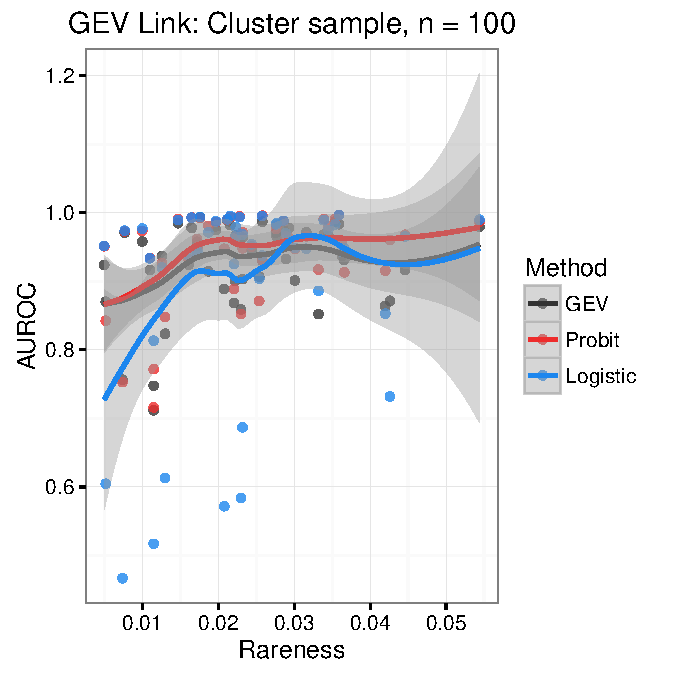
\includegraphics[width=0.47\linewidth]{byrareness-1}
  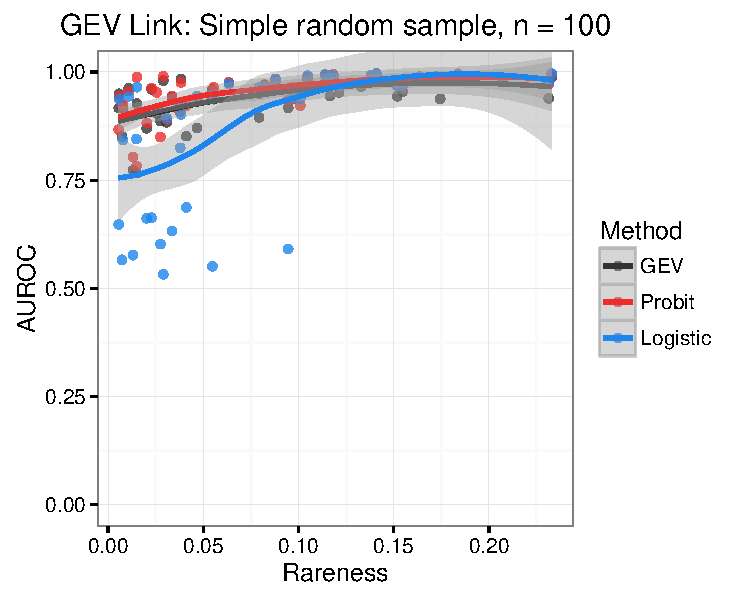
\includegraphics[width=0.47\linewidth]{byrareness-2}

  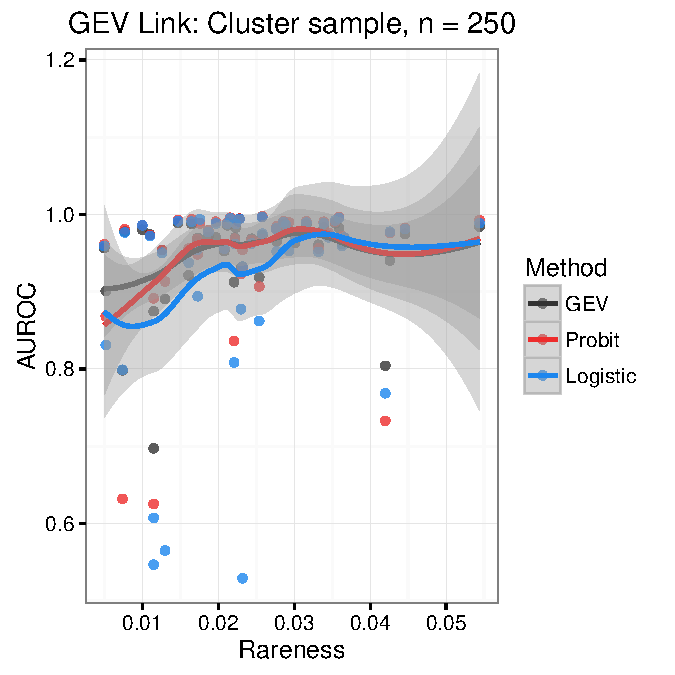
\includegraphics[width=0.47\linewidth]{byrareness-3}
  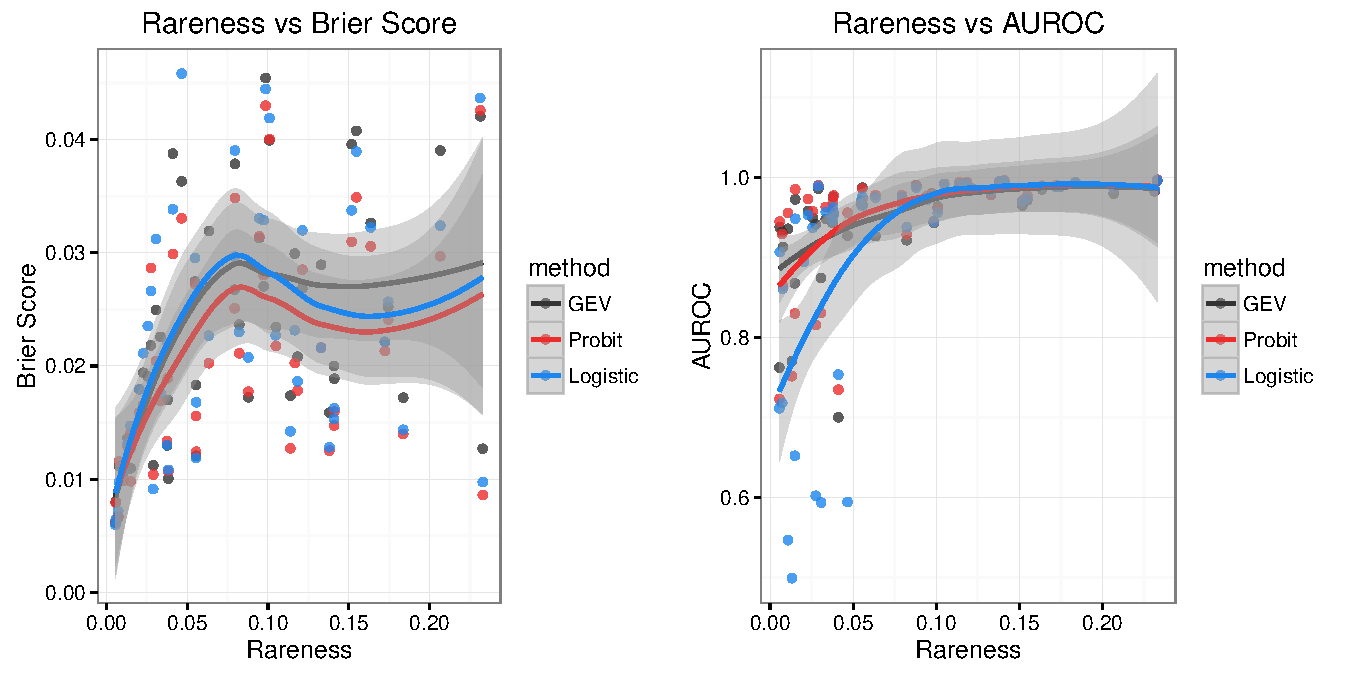
\includegraphics[width=0.47\linewidth]{byrareness-4}
  \caption{Smooth of AUROC by rareness for each sample technique for the GEV link.}
  \label{rbfig:simsmooth-gev}
\end{figure}

\begin{figure}[htbp]  % code/analysis/simstudy/combine-tables.R
  \centering
  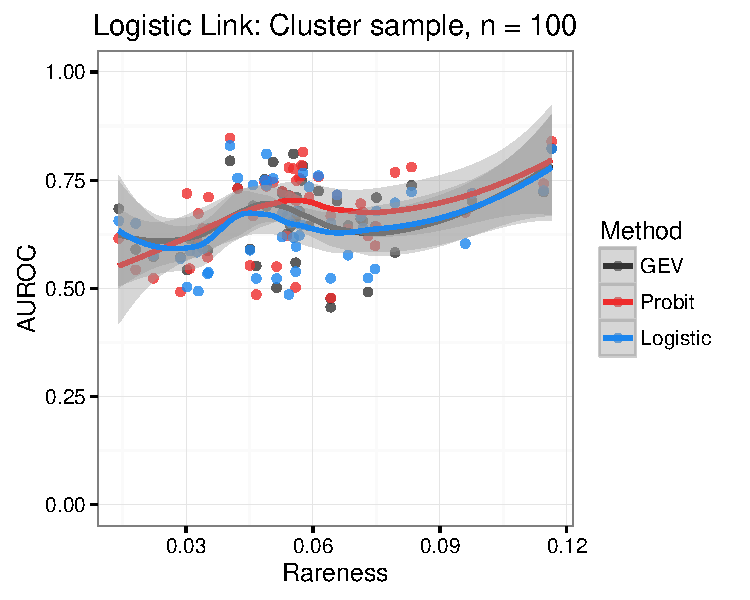
\includegraphics[width=0.47\linewidth]{byrareness-5}
  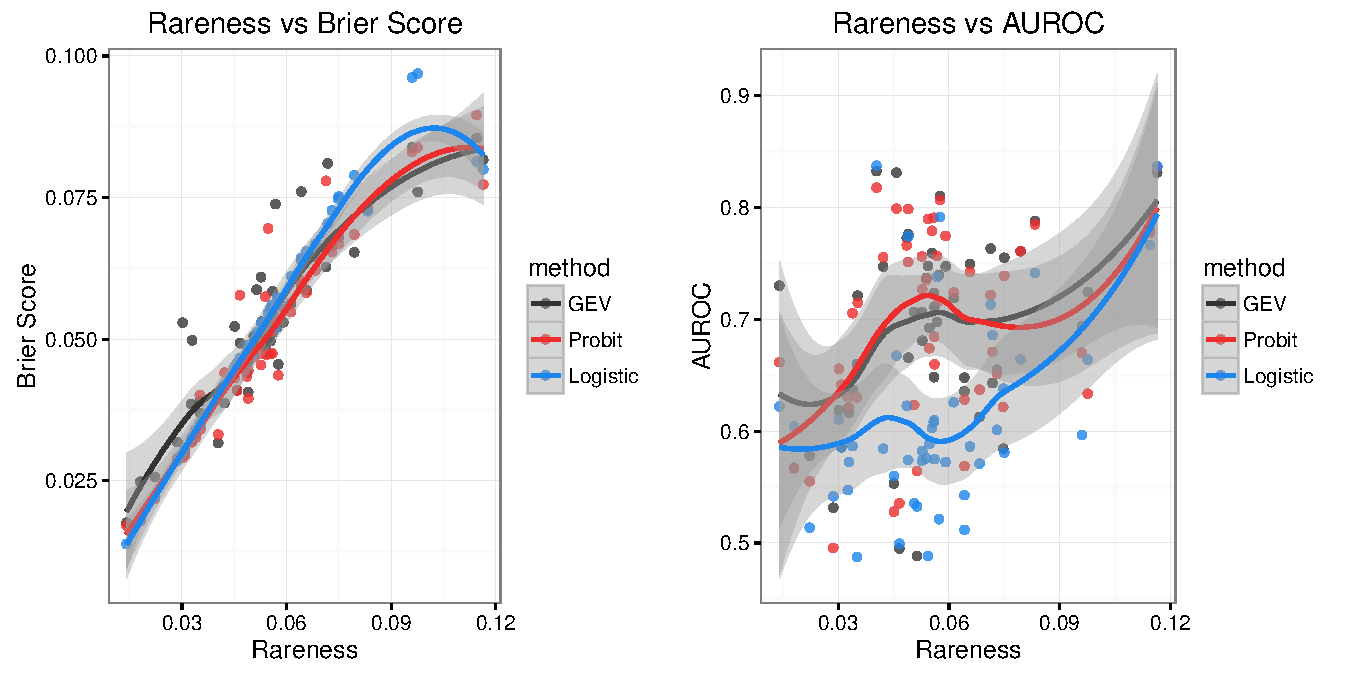
\includegraphics[width=0.47\linewidth]{byrareness-6}

  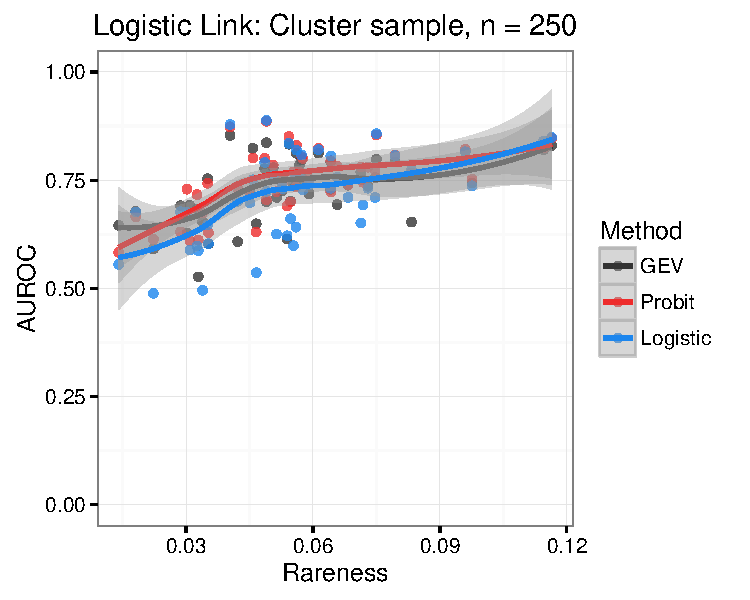
\includegraphics[width=0.47\linewidth]{byrareness-7}
  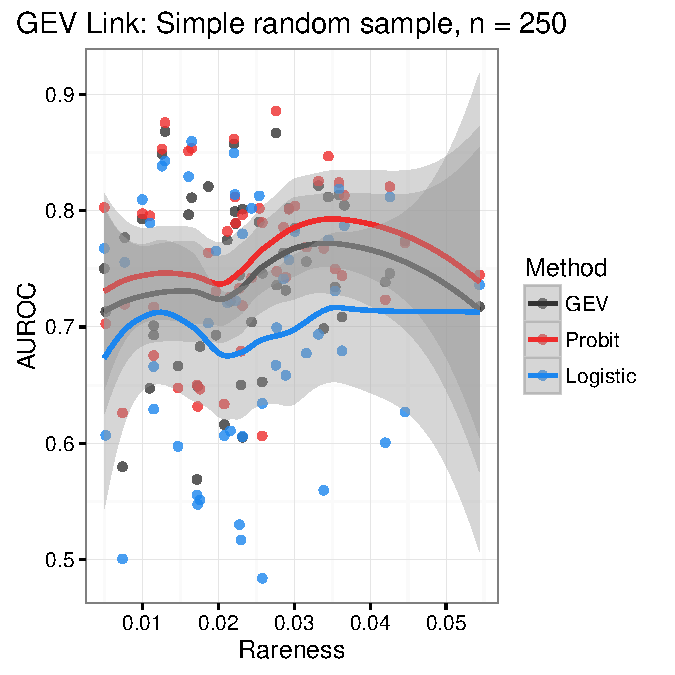
\includegraphics[width=0.47\linewidth]{byrareness-8}
  \caption{Smooth of AUROC by rareness for each sample technique for the logistic link.}
  \label{rbfig:simsmooth-log}
\end{figure}

\begin{figure}[htbp]  % code/analysis/simstudy/combine-tables.R
  \centering
  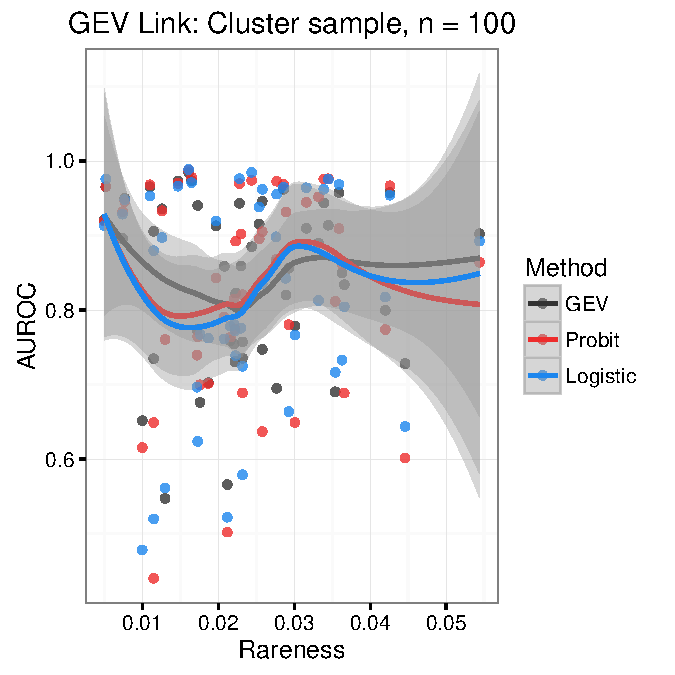
\includegraphics[width=0.47\linewidth]{byrareness-9}
  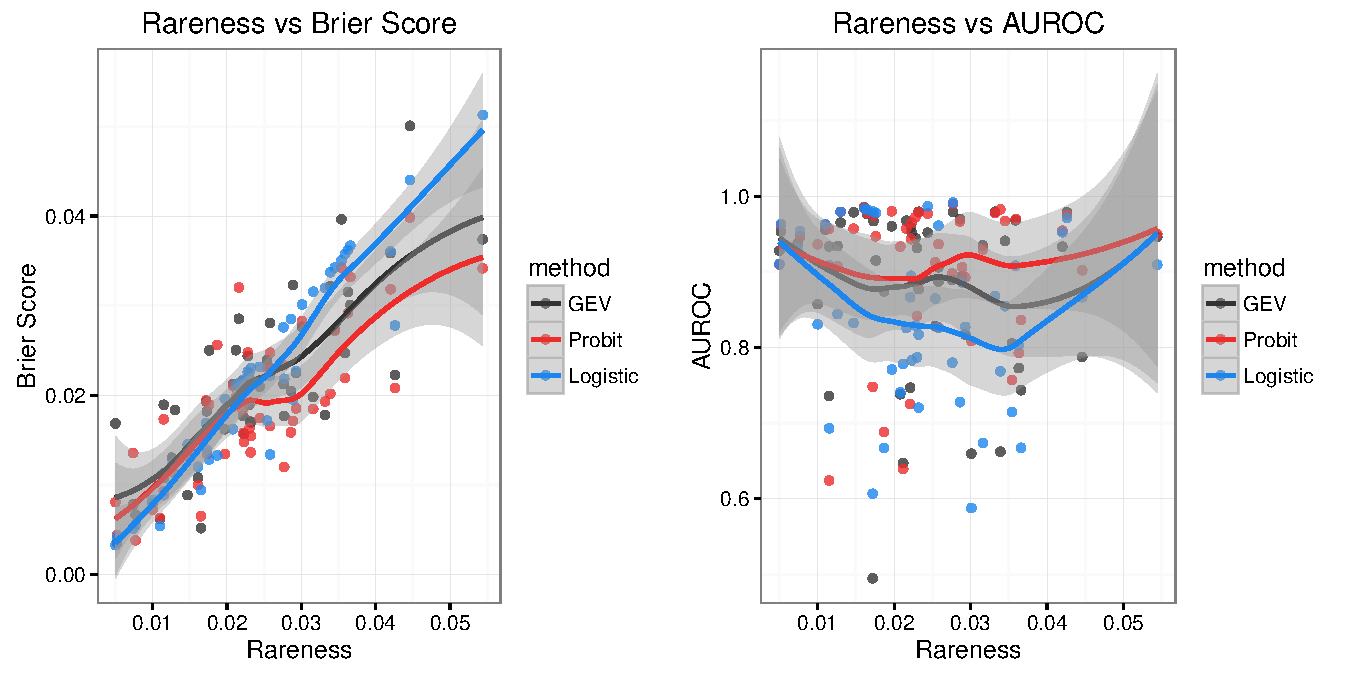
\includegraphics[width=0.47\linewidth]{byrareness-10}

  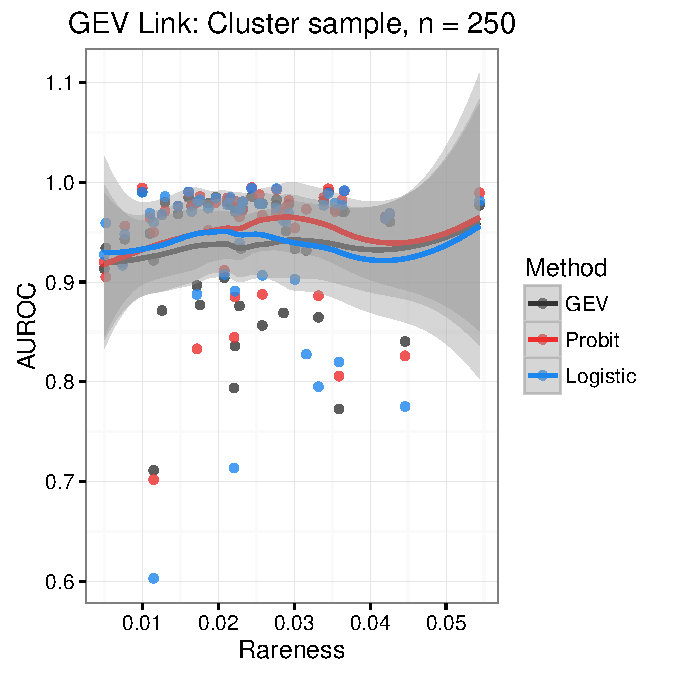
\includegraphics[width=0.47\linewidth]{byrareness-11}
  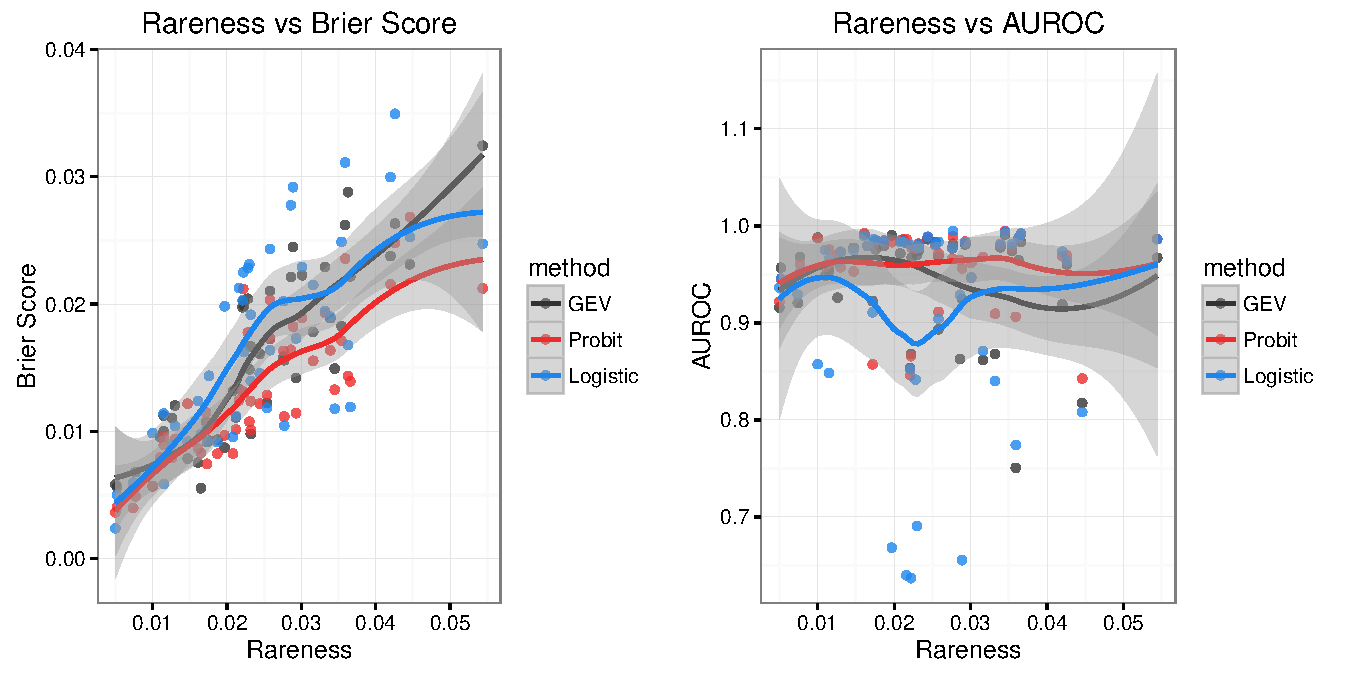
\includegraphics[width=0.47\linewidth]{byrareness-12}
  \caption{Smooth of AUROC by rareness for each sample technique for the hotspot link.}
  \label{rbfig:simsmooth-hot}
\end{figure}

\end{document}